\subsubsection{Pengujian operasi dasar}
\label{subsubsection:pengujian-operasi-dasar}

Pengujian ini mencakup fungsional F-1, yaitu bahwa sistem harus dapat melakukan operasi \textit{read} dan \textit{write} pada sebuah \textit{key-value store database}. Pengujian ini menggunakan \textit{script} pembantu oneshot.js yang sudah dijelaskan pada bagian \ref{subsubsection:implementasi-benchmark}. Implementasi dari oneshot.js dapat dilihat pada gambar \ref{fig:implementasi-oneshot}. 

\begin{figure}[ht]
    \centering
    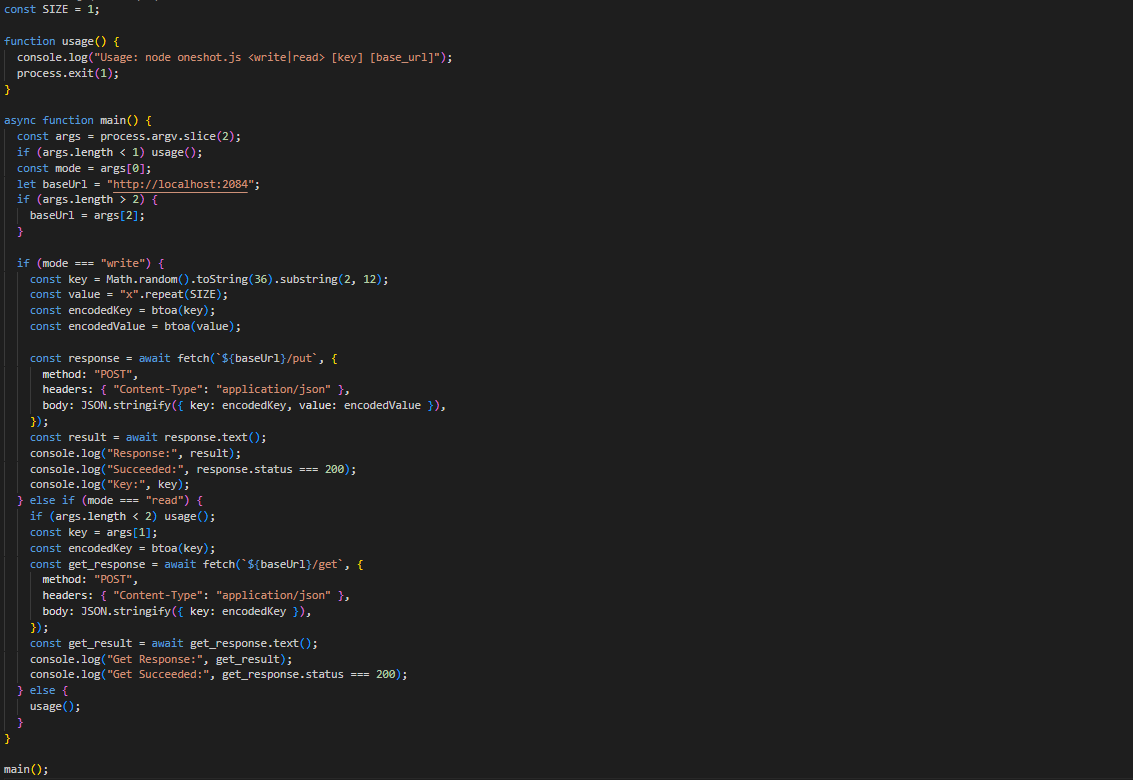
\includegraphics[width=0.95\textwidth]{resources/chapter-4/oneshot.png}
    \caption{Implementasi oneshot.js}
    \label{fig:implementasi-oneshot}
\end{figure}

Pengujian dibagi dua menjadi pengujian operasi \textit{write} dan \textit{read}. Kode dari pengujian tersebut adalah P-1 dan P-2. Pemetaan dapat dilihat pada lampiran \ref{appendix:pemetaan-pengujian}.

Pengujian operasi \textit{write} dengan kode pengujian P-1 dilakukan dengan skenario pengguna menuliskan \textit{key-value pair} ke dalam sistem. Nilai \textit{key} dan \textit{value} akan bersifat acak. Pengujian dilakukan dengan langkah-langkah sebagai berikut:

\begin{enumerate}
  \item Menunggu hingga sistem siap menerima \textit{request}. Konfirmasi dapat dilakukan dengan mengirim \textit{request} HTTP pada \textit{endpoint} /status dan memastikan bahwa sistem sudah memiliki \textit{leader}.
  \item Menjalankan \textit{script} oneshot.js dengan argumen \textit{write} untuk melakukan pengujian operasi dasar. \textit{Script} ini akan mengirimkan \textit{request} \textit{write} ke sistem.
  \item Mengirim request HTTP pada \textit{endpoint} /log untuk memastikan bahwa sistem telah menerima \textit{request} \textit{write} dan telah menyimpan data yang dituliskan.
  \item Mengulangi pengujian dengan sistem \textit{erasure coding} dan juga dengan sistem replikasi.
\end{enumerate}

Hasil yang diharapkan setelah tes dijalankan adalah sistem menyimpan \textit{log} yang berisi \textit{key-value pair} yang telah dituliskan. Untuk \textit{erasure coding}, log yang disimpan harus berisi \textit{key-value pair} yang telah di-\textit{encode} sesuai dengan konfigurasi yang telah ditentukan serta berbeda-beda untuk setiap \textit{node} sesuai dengan index \textit{fragment} yang diterima.

Pengujian operasi \textit{read} dengan kode pengujian P-2 dilakukan dengan skenario pengguna membaca \textit{key-value pair} yang sudah dituliskan sebelumnya. Pengujian dilakukan dengan langkah-langkah sebagai berikut:

\begin{enumerate}
  \item Menunggu hingga sistem siap menerima \textit{request}. Konfirmasi dapat dilakukan dengan mengirim \textit{request} HTTP pada \textit{endpoint} /status dan memastikan bahwa sistem sudah memiliki \textit{leader}.
  \item Menjalankan \textit{script} oneshot.js dengan argumen \textit{read} untuk melakukan pengujian operasi dasar. \textit{Script} ini akan mengirimkan \textit{request} \textit{read} ke sistem.
  \item Mengirim request HTTP pada \textit{endpoint} /log untuk memastikan bahwa sistem mengembalikan nilai \textit{request} \textit{read} yang sesuai dengan nilai yang disimpan pada \textit{log}.
  \item Mengulangi pengujian dengan sistem \textit{erasure coding} dan juga dengan sistem replikasi.
\end{enumerate}

Hasil yang diharapkan setelah tes dijalankan adalah sistem mengembalikan nilai \textit{key-value pair} yang telah dituliskan sebelumnya. Untuk \textit{erasure coding}, sistem harus dapat mengembalikan nilai \textit{key-value pair} yang utuh dan bukan nilai \textit{fragment} yang di-\textit{encode}.